\subsection{Системы небесных координат}
\term{Горизонтальная система координат}~--- система координат, в которой основной плоскостью является плоскость математического горизонта, а полюсами~--- зенит и надир. Одной координатой является либо \term{высота светила} $h$, либо его {зинитное расстояние} $z$. Другой координатой является \term{азимут} $A$, отсчитываемой от точки юга.


\begin{figure}[!h]
\begin{center}
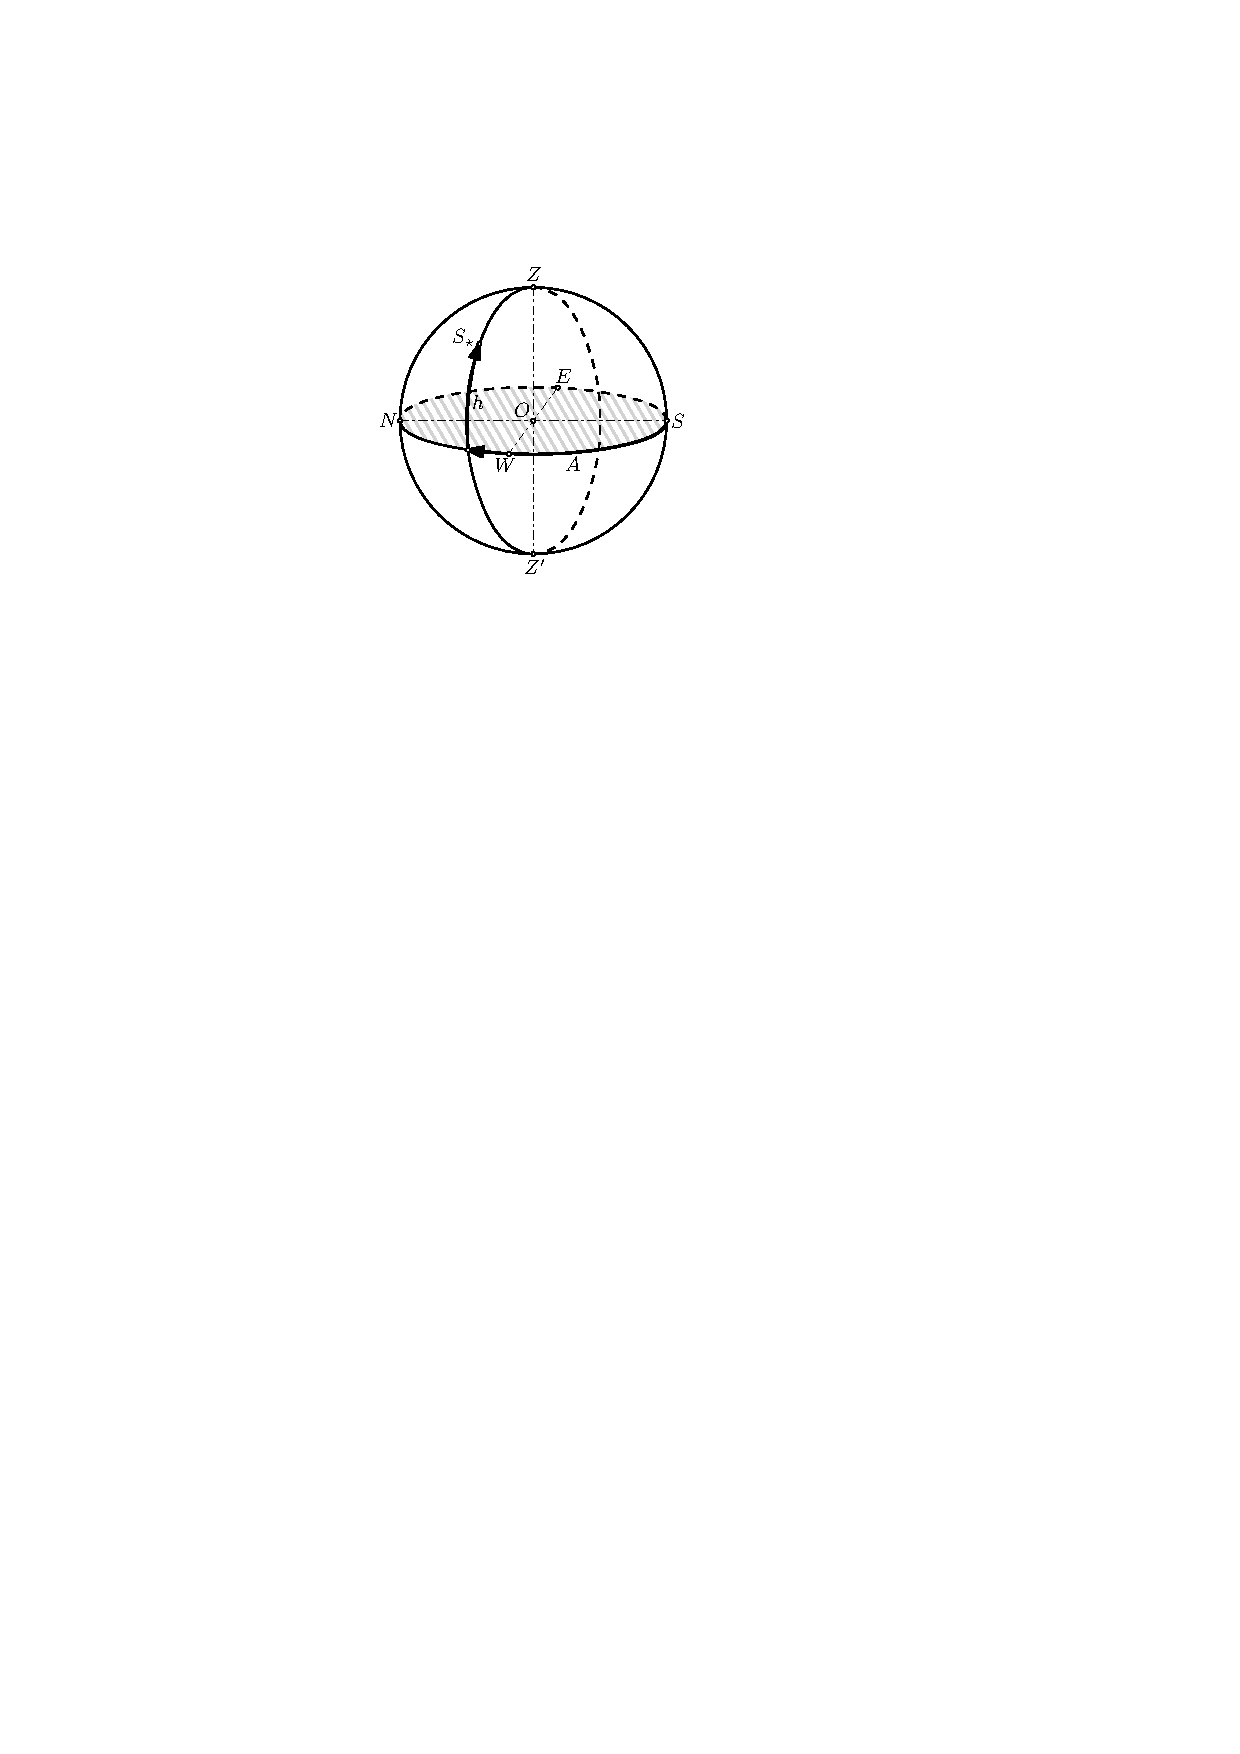
\includegraphics[width=0.5\textwidth]{hor-coordin-sys}
\caption{Горизонтальная система координат}
\end{center}
\end{figure}

\term{Первая экваториальная система координат}~--- система координат, основной плоскостью которой является плоскость небесного экватора. Одной координатой при этом является \term{склонение} $\delta$ (реже~--- \term{полярное расстояние} $p$). Другой координатой~--- \term{часовой угол} $t$~--- дуга небесного экватора от верхней точки небесного экватора до круга склонения светила, или двугранный угол между плоскостями небесного меридиана и круга склонения светила.

\term{Вторая экваториальная система координат}~--- система, основной плоскостью которой является плоскость небесного экватора. Одна координата~--- \term{склонение} $\delta$. Другой координатой является \term{прямое восхождение} $\alpha$.


\begin{figure}[!h]
\begin{center}
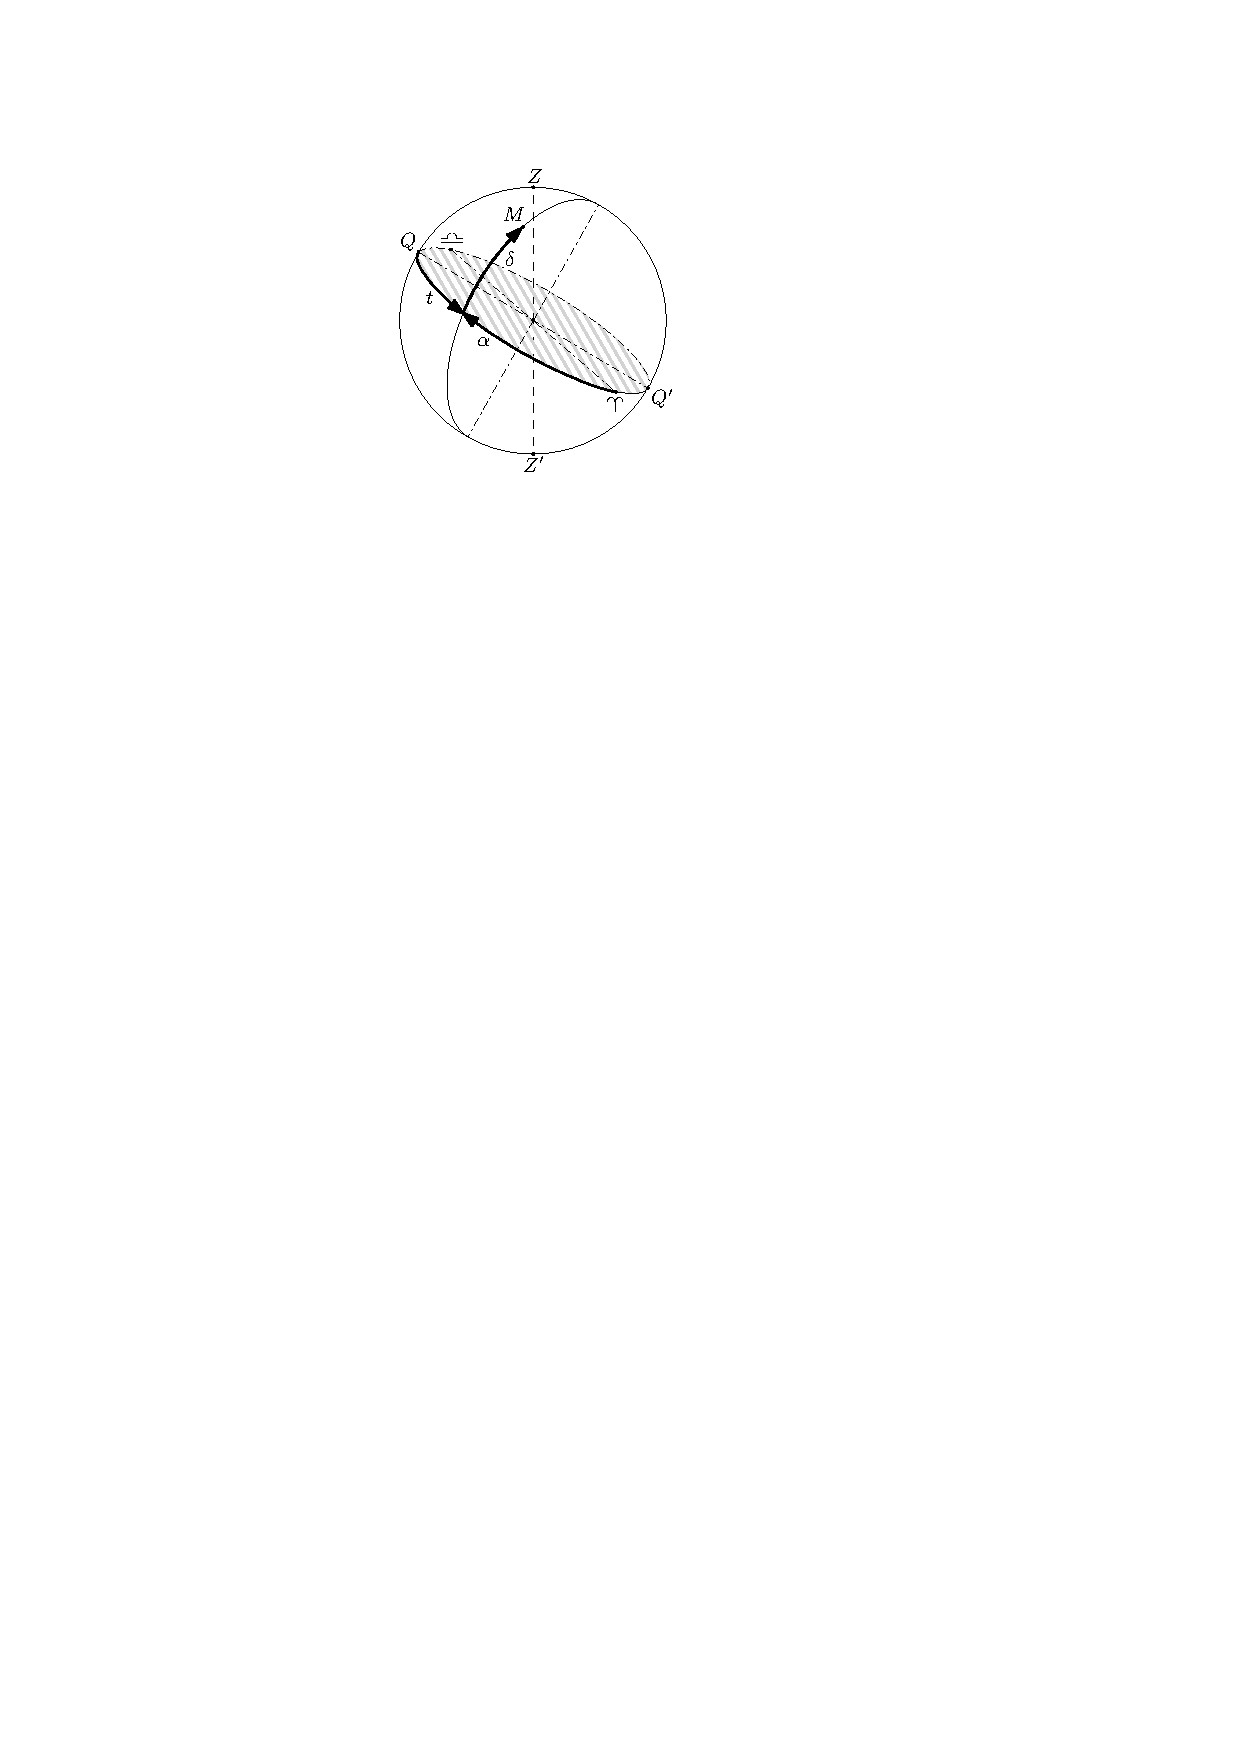
\includegraphics[width=0.5\textwidth]{eq-coordin-sys}
\caption{Экваториальная система координат}
\end{center}
\end{figure}

\term{Эклиптическая система координат}~--- система координат, основной плоскостью которой является плоскость эклиптики. Одной координатой при этом является \term{эклиптическая широта} $\beta$, а другой~--- \term{эклиптическая долгота} $\lambda$.

\begin{figure}[!h]
\begin{center}
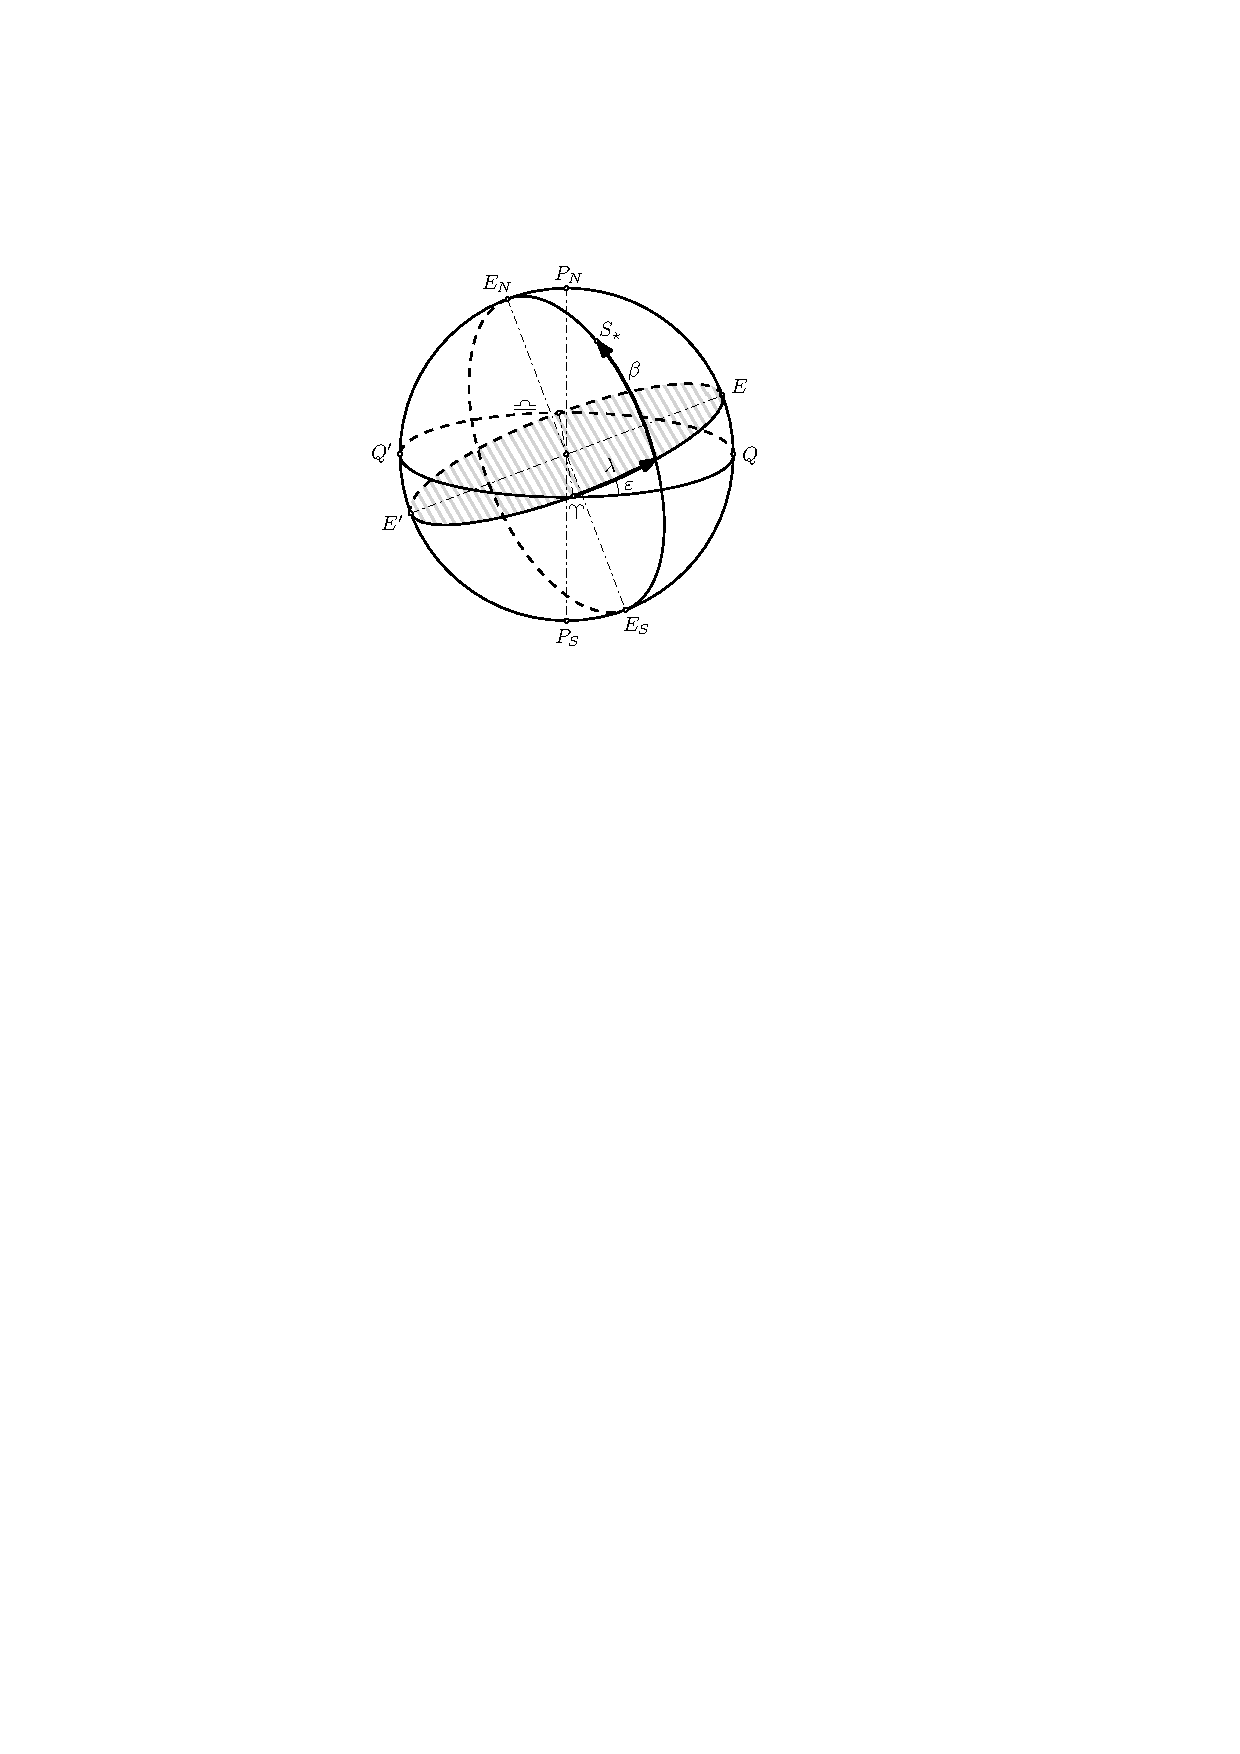
\includegraphics[width=0.5\textwidth]{eql-coordin-sys}
\caption{Эклиптическая система координат}
\end{center}
\end{figure}

\term{Галактическая система координат}~--- система координат основной плоскостью которой является плоскость нашей Галактики, которая наклонена к плоскости экватора под углом $62.6^{\circ}$. Одной координатой при этом является \term{галактическая широта} $b$~--- дуга круга галактической широты от эклиптики до светила, или угол между плоскостью галактического экватора и направлением на светило, а другой~--- \term{галактическая долгота} $l$~--- дуга галактического экватора от точки начала отсчёта $C$ до круга галактической широты светила, или угол между направлением на точку начала отсчёта $C$ и плоскостью круга галактической широты светила. Точка $C$ примерно совпадает с направлением на центр галактики и имеет координаты: $\alpha=17^h45^m.6$; $\delta=-28^{\circ}56'.2$ $G_NG_S$~--- плоскость галактического экватора, $QQ'$~--- плоскость небесного экватора, $M$~--- светило, $P_NP_S$~--- ось мира. $\aries$ и $\libra$~--- точки весеннего и осеннего равноденствия соответственно.

\begin{figure}[!h]
\begin{center}
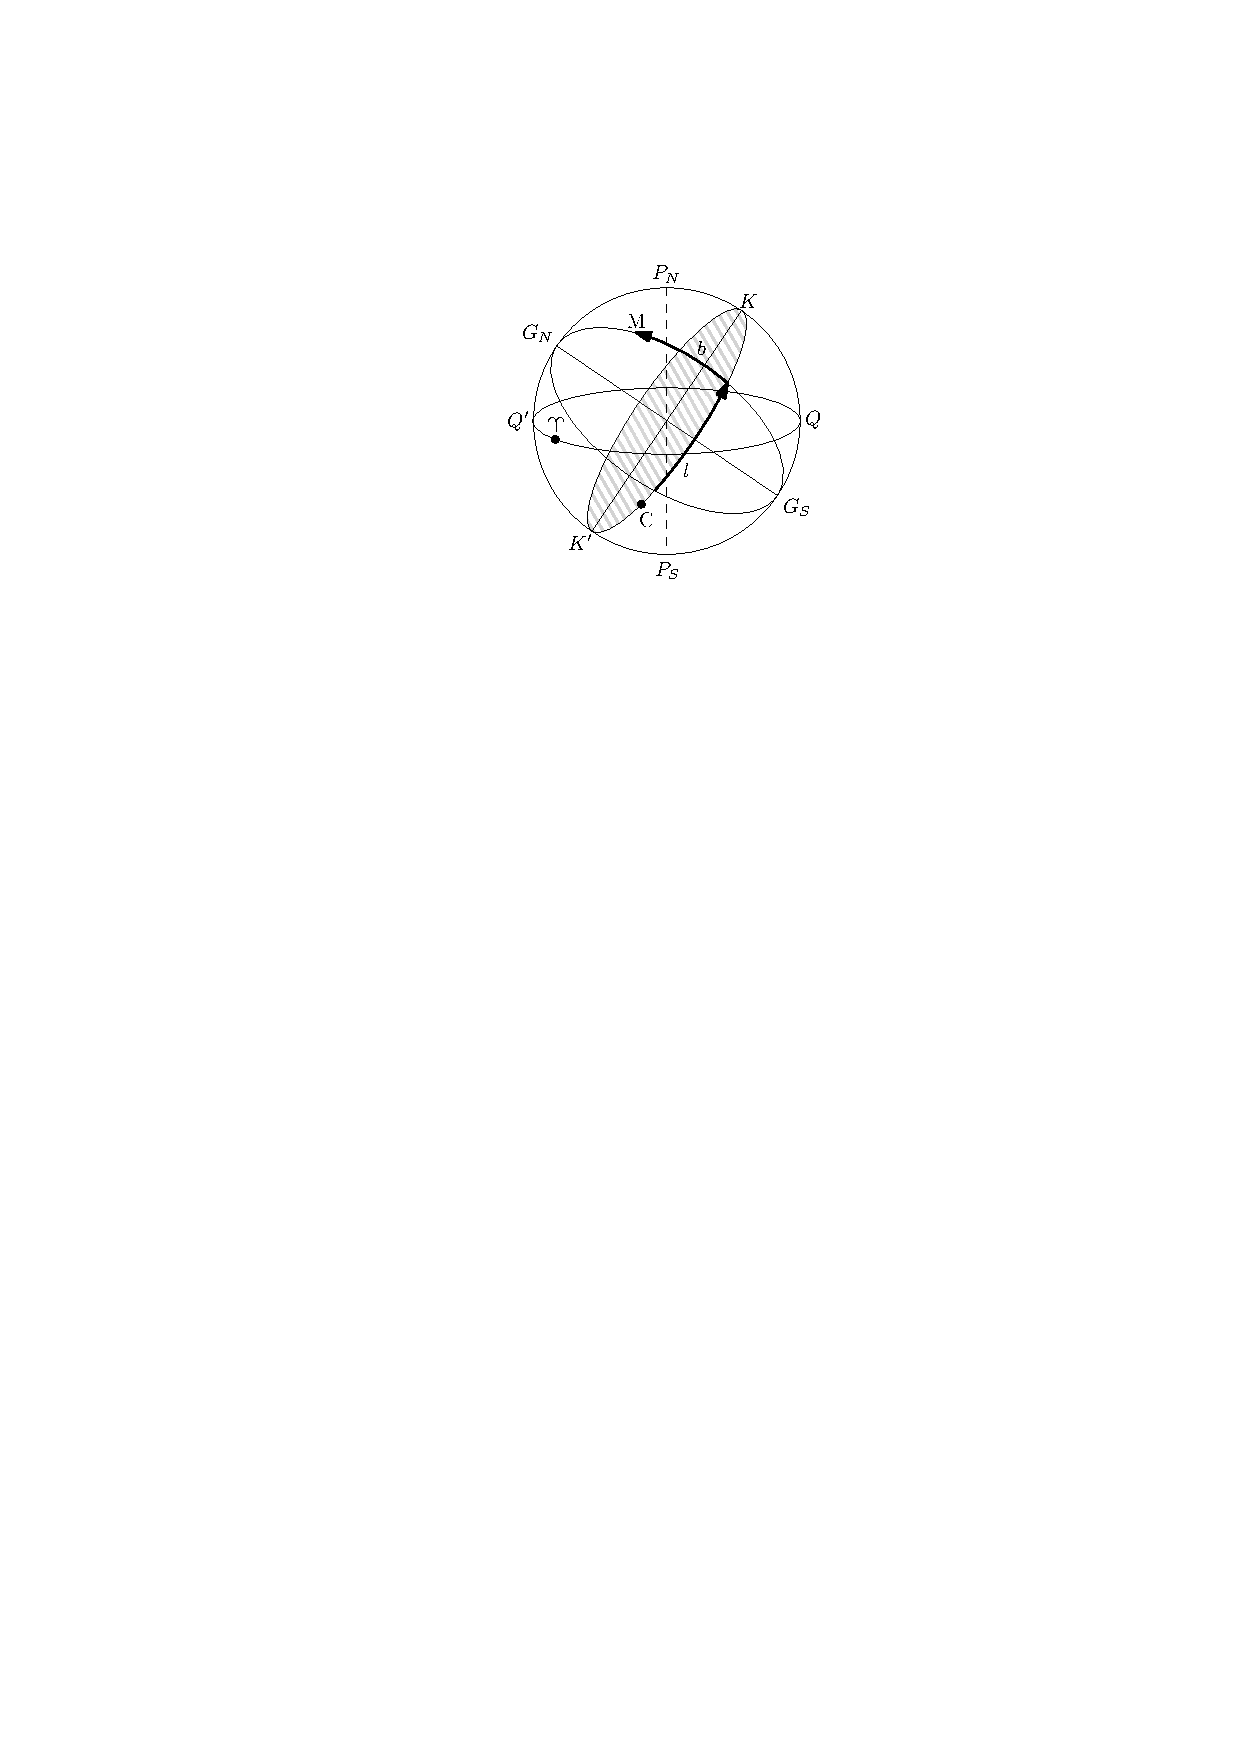
\includegraphics[width=0.5\textwidth]{gal-coordin-sys}
\caption{Галактическая система координат}
\end{center}
\end{figure}